\documentclass[a4paper]{article}

%% Language and font encodings
\usepackage{polski}
\usepackage[polish]{babel}
\usepackage[utf8x]{inputenc}
\usepackage[T1]{fontenc}
\usepackage{pdfpages}
\usepackage{indentfirst}
\usepackage{listings}
\usepackage{gensymb}

% Adjust penalties
\brokenpenalty=1000
\clubpenalty=1000
\widowpenalty=1000

%% Sets page size and margins
\usepackage[a4paper]{geometry}

%% Useful packages
\usepackage{amsmath}
\usepackage{graphicx}
\usepackage[colorlinks=true, allcolors=blue]{hyperref}
\usepackage{booktabs}
\usepackage{cancel}
\usepackage{tikz}

\usepackage{float}

\renewcommand\thesection{\arabic{section}.}
\renewcommand\thesubsection{\arabic{section}.\arabic{subsection}.}
\renewcommand\thesubsubsection{\arabic{section}.\arabic{subsection}.\arabic{subsubsection}.}

% The following commands are not supported in PSTricks at present
% We define them conditionally, so when they are implemented,
% this pgf file will use them.
\ifx\du\undefined
  \newlength{\du}
\fi
\setlength{\du}{15\unitlength}

\newcommand{\Vsp}[1]{\vtop to #1 {}}
\newcommand{\Hsp}[1]{\hbox to #1 {}}
\newcommand{\Small}{\scriptsize}

\title{Sprawozdanie nr 4}
\date{}

\begin{document}

\begin{center}
\begin{tabular}{|p{5cm}|l|l|l|}
    \hline
    Wydział \Vsp{5mm} & \multicolumn{1}{|l}{Dzień} &  & Nr zespołu\\
    & \multicolumn{1}{|l}{Data} &  & \\
    \hline 
    Nazwisko i Imię: & \Small Ocena z przygotowania  & \Small Ocena ze sprawozdania & \Small Ocena Końcowa \\
    1. & & &\\
    2. & & & \\
    3. & & & \\
    \hline
    \multicolumn{2}{|l|}{Prowadzący \Vsp{1cm}} & \multicolumn{2}{|l|}{Podpis prowadzącego} \\
    \hline
\end{tabular}
\end{center}

{\let\newpage\relax\maketitle}
\setcounter{secnumdepth}{2}
\setcounter{tocdepth}{2}

\section{Interferencja fal} %TODO może lepsza nazwa

\subsection{Opis ćwiczenia}

Celem ćwiczenia jest pomiar długości fal elektromagnetycznych metodami interferencyjnymi.
Wykorzystujemy do tego następujące przyrządy:
\begin{itemize}
\item interferometr Michelsona
\item interferometr Fabry-Perota
\item siatkę dyfrakcyjną
\end{itemize}
W eksperymentach zostały wykorzystane mikrofale oraz światło widzialne w postaci lasera o kolorze czerwonym.

\subsection{Wstęp teoretyczny}

\subsubsection{Interferencja}

Interferencja jest efektem nakładania się fal. W wyniku nałożenia może nastąpić wzmocnienie fali wypadkowej lub jej osłabienie.  Warunkiem trwałej interferencji fal jest ich spójność, czyli korelacja faz i równość częstotliwości. W przeciwnym wypadku może dość np. do dudnienia. %TODO może usunąć dudnienie
Fale powinny też posiadać identyczną częstość kołową w i mieć taką samą polaryzację.
Natężenia nakładających się fal opisane są wzorami
$$E_{1} = E_{01} sin( \omega t − kx )$$
$$E_{2} = E_{02} sin( \omega t − k ( x + \Delta ))$$

gdzie dla fali drugiej przebywa ona dodatkową drogę $\Delta$ która powoduje różnicę w fazach pomiędzy falami.

Podczas interferencji czyli dodaniu się fal otrzymujemy następującą zależność
$$E = E_{1} + E_{2} = E_{01} sin( \omega t − kx ) + E_{02} sin( \omega t − k x  − \phi )$$ gdzie $\phi =\frac{2\pi}{\lambda}\Delta$ - opisuje zmianę fazy spowodowaną przebyciem dodatkowej drogi optycznej.

Używane przez nas detektory reagują na średnią ilość energii padającej na jednostkę powierzchni w jednostce czasu. Energia fali jest proporcjonalna do kwadratu natężenia pola elektrycznego, zależność tą możemy otrzymać z poprzedniego wzoru wynosi ona:
$$E^2 = ( E_{1} + E_{2} ) = E_{01}^2 sin^2 ( \omega t − kx ) + E_{02}^2 sin^2 ( \omega t − kx − \phi ) + 2 E_{01} E_{02} sin( \omega t − kx ) sin( \omega t − kx − \phi )$$

Z czego po odpowiednich przekształceniach otrzymujemy 
$$E^2 = E_{01}^2 sin^2 (\omega t − kx ) + E_{02}^2 sin^2 ( \omega t − kx − \phi ) + E_{01} E_{02} [cos \phi − cos[ 2 ( \omega t − kx ) − \phi ]]$$

Mając powyższą zależność możemy wyznaczyć wcześniej wspomnianą średnią ilość energii na jednostę powierzchni
$$I = E^2 =\frac{E_{01}}{2} \frac{E_{02}}{2} + E_{01}E_{02} cos \phi$$

Ostatecznie otrzymując 
$$I = I_{1} + I_{2} + 2 \sqrt{I_{1} I_{2}} cos \phi$$

co dla przypadku przez nas badanego $I_{1} = I_{2}$ sprowadza się do związku
$$I = 2I_{0} + 2 I_{0} cos \phi$$

w zależności od kąta przesunięcia fazowego $\phi =\frac{2\pi}{\lambda}\Delta$ otrzymujemy $0$ lub $4 I_{0}$ bo $cos \phi$ odpowiednio osiąga wartości $-1$ lub $1$. Z powyższych rozważań wynikia ostatecznie że 
$\lambda = 2 \frac{\Delta}{2m+1} $ dla osłabienia oraz $\lambda = \frac{\Delta}{m}$ dla wzmocnienia.

\newpage

\subsection{Siatka dyfrakcyjna}
\begin{figure}[h]
\centering
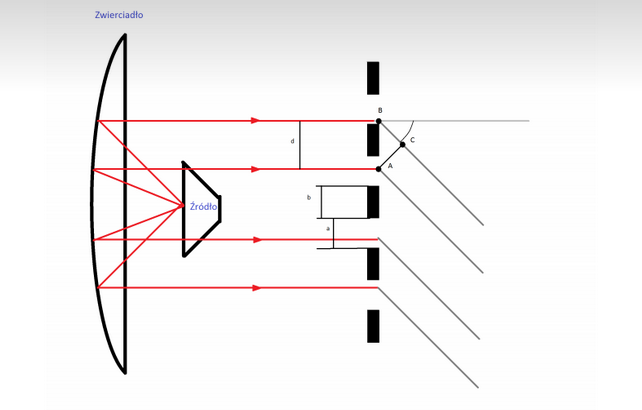
\includegraphics[scale=0.4]{siatka_dyfrakcyjna_rysunek.png}
\caption{Schemat układu pomiarowego dla siatki dyfrakcyjnej}
\label{siatka_dyfrakcyjna}
\end{figure}

\begin{figure}[h]
\centering
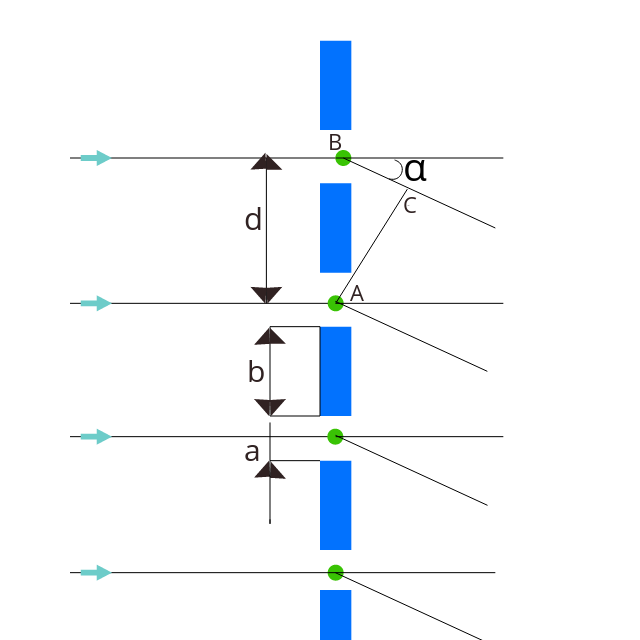
\includegraphics[scale=0.4]{siatka.png}
\caption{Schemat układu pomiarowego dla siatki dyfrakcyjnej}
\label{siatka}
\end{figure}


Do przeprowadzenia eksperymentu z siatką dyfrakcyjną posłużono się układem widocznym na rysunku \ref{siatka_dyfrakcyjna}. Źródło mikrofal które znajdowało się w odległości $\frac{1}{2}$ promienia krzywizny
zwierciadła wysyłało fale elektromagnetyczne które odbijały się od zwierciadła. Dzięki temu osiągaliśmy równoległe fale elektromagnetyczne. Następnie przechodziły przez szczeliny siatki dyfrakcyjnej
i zgodnie z zasadą Huyghensa były one wtórnymi źródłami fal kulistych które ze sobą interferowały dając minima oraz maksima sygnału obserwowanego na woltomierzu w miejsach o odpowiednich kątach względem siatki dyfrakcyjnej w których znajdował się odbiornik fal.
Na siatce dyfrakcyjnej dochodzi do powstania fal rozchodzących się kuliście jeśli różnica dróg widoczna na rysunku \ref{siatka} wynosi $d sin \alpha_{m} = m \lambda$ wówczas dochodzi do maksymalnego wzmocnienia fali wynikowej.

Otrzymano następujące wyniki:

\begin{table}
\centering
\begin{tabular}{rrrrrrr}
\toprule
Lp. &  $\alpha$ (\degree) \\
\midrule
1 &          0\\
2 &          26  \\
3 &          26 \\
4 &          53  \\
5 &          55  \\
\bottomrule
\end{tabular}
\caption{Wielokrotne pomiary prądu $I_{R_4}$ i napięcia $U_{R_4}$ na rezystorze $R_4$.}
\label{pomiary_siatka}
\end{table}



\subsection{Interferometr Michelsona - mikrofale}

\begin{figure}[h]
\centering
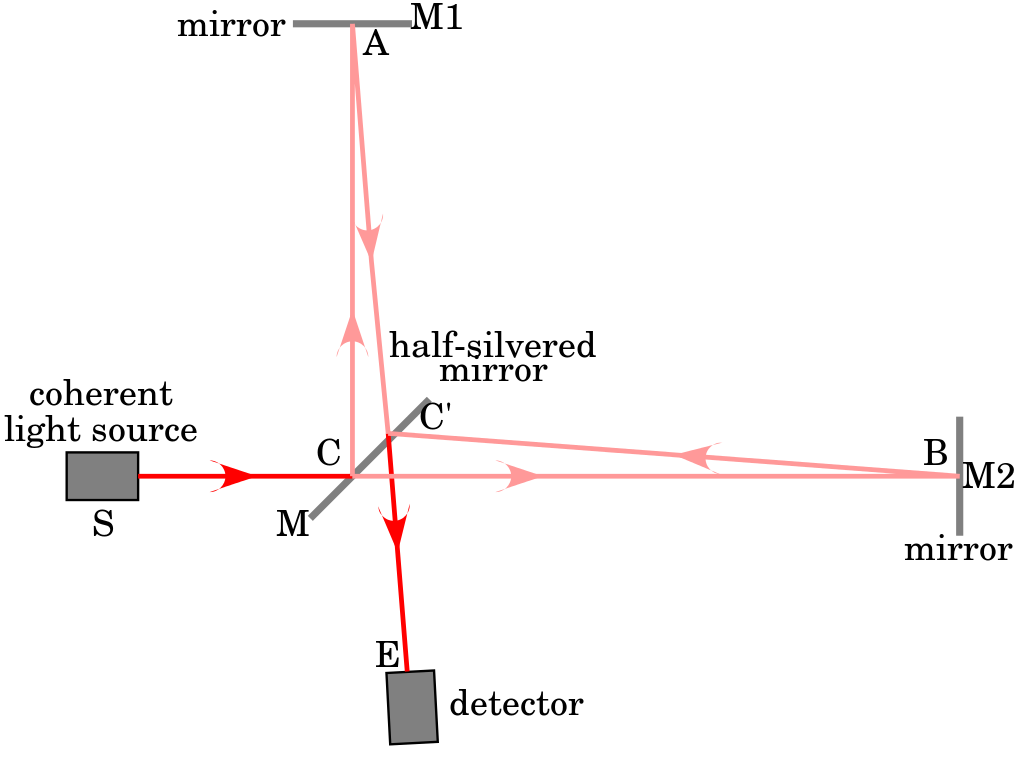
\includegraphics[scale=0.2]{Michelson_interferometer.png}
\caption{Schemat układu pomiarowego dla interferometru michelsona $https://upload.wikimedia.org/wikipedia/commons/thumb/d/d4/Michelson_interferometer_with_labels.svg/1024px-Michelson_interferometer_with_labels.svg.png$}
\label{michelson}
\end{figure}

 Wiązka mikrofal wychodzi ze źródła i pada na płytkę półprzepuszczlną. Połowa  wiązki odbija się od płytki pada na jedno ze zwierciadeł, odbija się i wraca tą samą drogą, przechodzi przez płytkę i pada na detektor.  Druga połowa wiązki przechodzi przez płytkę odbija się od drugiego zwierciadła i wraca tą samą drogą, odbija się od płytki, spotyka się z wiązką pierwszą w detektorze. Przesuwając jedno ze zwierciadeł zbadaliśmy ilość maksymalnych wzmocnień obserwowanych w detektorze oraz odległość na jakiej miało miejsce dane wzmocnienie. Wyniki zestawiliśmy w poniższej tabeli. 

\begin{table}
\centering
\begin{tabular}{rrrrrrr}
\toprule
Lp. &  odległość ($cm$) \\
\midrule
1 & 2 \\
2 & 3.7 \\
3 & 5.5 \\
4 & 7.3 \\
5 & 9.0 \\
6 & 10.8 \\
7 & 12.5 \\
8 & 14.2 \\
9 & 16.0 \\
10 & 17.7 \\
11 & 19.4 \\
12 & 21.2 \\
13 & 23.0 \\
14 & 24.7 \\
15 & 26.4 \\
16 & 28.2 \\
17 & 29.9 \\
\bottomrule
\end{tabular}
\caption{Wielokrotne pomiary prądu $I_{R_4}$ i napięcia $U_{R_4}$ na rezystorze $R_4$.}
\label{pomiary_siatka}
\end{table}


\subsection{Interferometr Fabry-Perot}
nterferometr Fabry – Perota składa się z dwóch płytek, jedna z nich przepuszcza część promieniowania, a druga ma zdolność do odbijania. Płytki ustawiamy tak aby, powietrze pomiędzy płytkami tworzyło płaskorównoległą warstwę. Fale, które przez górną płytkę przedostają się do warstwy powietrza, ulegają wielokrotnym odbiciom od ścianek płytek. Jeśli na pierwszą płytkę pada wiązka fal, to z drugiej płytki wychodzi szereg równoległych wiązek. Badaliśmy odległości pomiędzy płytkami P przy maksymalnym wzmocnieniu. Wyniki zestawiliśmy w poniższej tabeli. 

\begin{figure}[h]
\centering
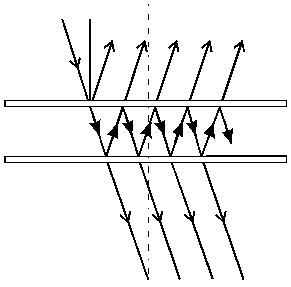
\includegraphics[scale=0.7]{fabry_perot.png}
\caption{Schemat układu pomiarowego dla interferometru Fabry-Perot $http://www.lodd.p.lodz.pl/~konrad/wyklad8/wyklad8/wyklad2.gif$}
\label{michelson}
\end{figure}

Wyniki zestawiliśmy w poniższej tabeli. 

\begin{table}
\centering
\begin{tabular}{rrrrrrr}
\toprule
Lp. &  odległość ($cm$) \\
\midrule
Numer maksimum,odległość (cm)
0 & 9.0 \\
18 & 38.9 \\
\bottomrule
\end{tabular}
\caption{Wielokrotne pomiary prądu $I_{R_4}$ i napięcia $U_{R_4}$ na rezystorze $R_4$.}
\label{pomiary_fabry_perot}
\end{table}




\end{document}
